\documentclass[runningheads]{venue/lncs/llncs}

\usepackage{amsmath,amssymb}
\usepackage{booktabs}
\usepackage{graphicx}
\usepackage{float}
\usepackage{microtype}
\usepackage[table]{xcolor}
\usepackage{url}
\usepackage{placeins}
\emergencystretch=2em
\setlength{\textfloatsep}{8pt plus 2pt minus 2pt}
\setlength{\floatsep}{8pt plus 2pt minus 2pt}
\setlength{\intextsep}{8pt plus 2pt minus 2pt}

\newcommand{\mae}{\operatorname{MAE}}
\newcommand{\rmse}{\operatorname{RMSE}}
\newcommand{\group}{\textsc{GROUP}}
\newcommand{\spatial}{\textsc{SPATIAL}}
\newcommand{\predkd}{\textsc{Prediction-KD}}

\title{When Transfer Accuracy Is Not Enough: Deployment-Conditioned Behavioural Diagnostics for Knowledge Transfer}
\titlerunning{Deployment-Conditioned Behavioural Diagnostics}
\author{Anonymous}
\authorrunning{Anon}
\institute{Anonymous Institution}

\begin{document}
\maketitle

\begin{abstract}
Crop-yield prediction informs agricultural planning and risk management, yet target regions often have few labels and uneven environmental measurements. Building a complete local dataset is costly and slow. Transfer learning and knowledge distillation (KD) can reuse external data, but source value may depend on the target population, spatial support, and deployment inputs. We introduce a deployment-conditioned evaluation that aligns local and transferred models within each contract and compares predictive error, common-sample attribution redistribution, and finite feature-group stress response. The study transfers from US maize to Australian wheat under GROUP and SPATIAL contracts, using target scratch, supervised transfer, and four KD routes. Under SPATIAL, prediction KD reaches a mean absolute error (MAE) of 0.954~t/ha, compared with 1.204 for scratch and 1.024 for supervised transfer. Under GROUP, the same route reaches 1.157~t/ha, compared with 0.729 for scratch. In one pooled setting, attribution movement is associated with matched error change; its direction varies across runs, and no corresponding association was detected in the other route--contract settings. In a Roseworthy no-soil comparison, supervised source-initialised fine-tuning remains at 0.465 while scratch reaches 0.499. Realised transfer is therefore a property of the model--target--adaptation--deployment relation, not of a checkpoint alone.
\keywords{knowledge transfer \and deployment shift \and crop-yield prediction \and feature attribution \and model evaluation}
\end{abstract}

\section{Introduction}

Crop-yield prediction supports planting decisions, risk management, and resource allocation. Statistical and machine-learning systems combine weather, soil, remote-sensing, and historical yield information across agricultural scales \cite{Kallenberg2026CYBench,Khaki2019DNNYield}. Their use in a new region depends on timely local labels and environmental measurements. These observations are expensive to collect and often cover fewer seasons or modalities than established production data.

External data and pretrained representations are therefore attractive. Agricultural adaptation can help when source and target conditions are compatible and target labels are limited \cite{Bohra2025KenyaTransfer,Priyatikanto2023MaizeAdaptation}. Here the source is US maize and the target is Australian wheat. They share a weather interface but differ in crop, geography, climate, and production environment. Australian wheat yields also vary across locations and seasons \cite{Brown2020AustralianWheat,Potgieter2002AustralianWheat}. A shared interface enables adaptation, while realised benefit remains deployment dependent.

Deployment-oriented partitions define different target populations. Random splits estimate interpolation within an observed pool. Group holdouts target new environments or administrative populations; spatial blocks target new locations. Structured validation can change generalisation estimates and model selection \cite{Meyer2021AOA,Meyer2022MLMaps,Roberts2017StructuredCV}. The same checkpoint faces different extrapolation demands under these contracts. A local target learner is needed to identify added value or negative transfer \cite{Wang2019NegativeTransfer}.

Earlier heterogeneous comparisons with conventional baselines inspired by the CY-Bench crop-yield benchmark showed that model selection can change when the partition changes. For example, a model selected under interpolation was not always selected under an environment, spatial, or temporal holdout. These observations motivate the primary study. We therefore ask whether transfer benefit reverses across contracts, whether attribution shifts track matched error, whether stress and attribution produce similar rankings, and whether narrowing the available modalities changes relative value.

Aggregate error answers whether prediction improves, while attribution and controlled stress tests examine how the fitted function uses and responds to its inputs. Explanation-shift research studies attribution distributions, but less often aligns them with target-error differences on the same samples \cite{Kulinski2023ExplainingShift,Mougan2025ExplanationShift}. The stability of these relations across deployment contracts remains unclear.

We address this gap with three linked contributions. First, we evaluate realised transfer under GROUP and SPATIAL contracts against both local scratch and run-matched supervised transfer. Second, we align routes on common target samples and compare error, attribution redistribution, and finite stress response as complementary behavioural diagnostics. Third, we show empirically that prediction KD changes from positive to negative transfer across contracts, while the relations among behavioural views are not contract invariant.

\section{Method}

The method separates the deployment question, model construction, and observation layer (Fig.~\ref{fig:design}). Local and transferred models use the same target labels and evaluation rows within each contract. Source routes affect checkpoint construction only; all target adaptation is supervised.

\begin{figure}[t]
\centering
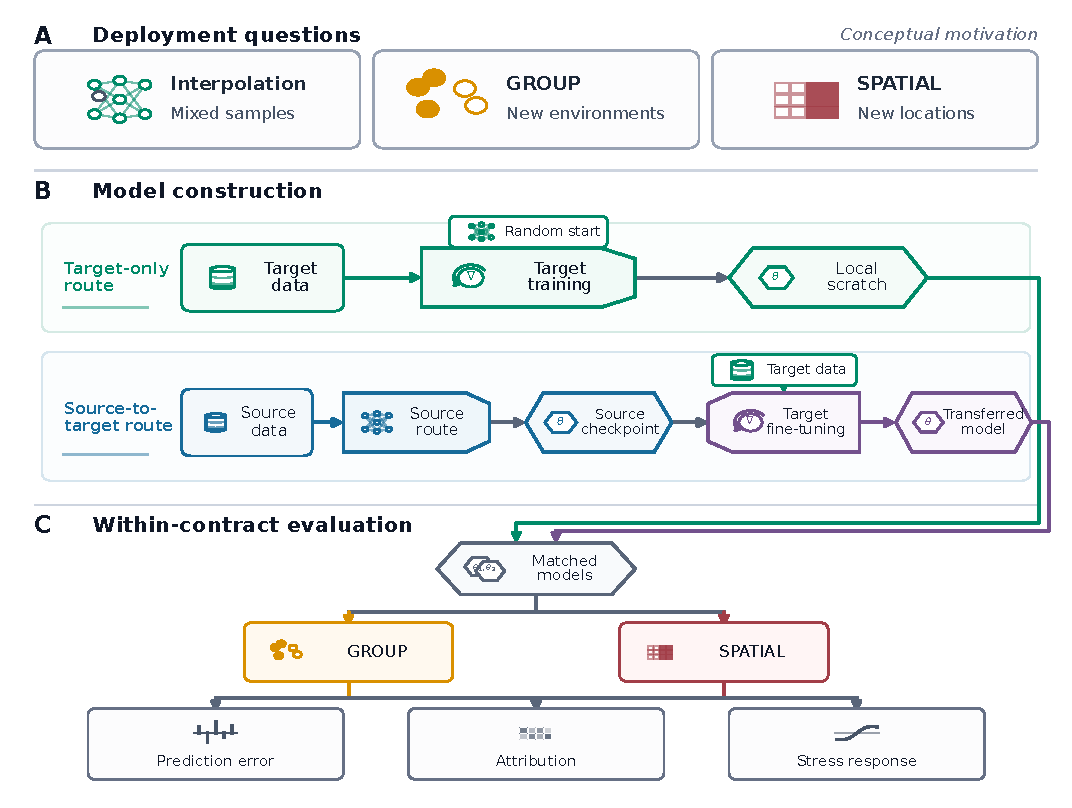
\includegraphics[width=.98\textwidth]{../figures/final_publication_v4_18/figure_01.pdf}
\caption{Study design. The conceptual top layer distinguishes interpolation, new environments, and new locations. The middle layer contrasts target-only training with source-route pretraining followed by supervised target fine-tuning. The lower layer compares local and transferred models within GROUP and SPATIAL using predictive error, attribution redistribution, and finite stress response.}
\label{fig:design}
\end{figure}
\FloatBarrier

We write a deployment contract as
\begin{equation}
\label{eq:contract}
\mathcal{C}=(\mathcal{D}_{s},\mathcal{D}_{t},\mathcal{S},\mathcal{M}_{\mathrm{train}},\mathcal{M}_{\mathrm{deploy}},\mathcal{A}),
\end{equation}
where source and target domains are $\mathcal{D}_{s}$ and $\mathcal{D}_{t}$, $\mathcal{S}$ defines the held-out target population, $\mathcal{M}$ specifies available inputs, and $\mathcal{A}$ is supervised target adaptation. The contract determines both the target support and the question a measured error can answer.

For route $r$, contract $c$, run $s$, target sample $i$, feature $j$, and feature group $G$, $f_{r,c,s}$ is the adapted target model. Source routes differ only before target adaptation. With frozen teacher $f_T$, student $f_\theta$, and representations $h_T,h_\theta$, the four mean squared error (MSE) terms are
\begin{equation}
\label{eq:component-losses}
\begin{aligned}
\mathcal{L}_{\rm sup}&=\operatorname{MSE}(f_\theta(\mathbf{x}),y), &
\mathcal{L}_{\rm pred}&=\operatorname{MSE}(f_\theta(\mathbf{x}),f_T(\mathbf{x})),\\
\mathcal{L}_{\rm repr}&=\operatorname{MSE}(h_\theta(\mathbf{x}),h_T(\mathbf{x})), &
\mathcal{L}_{\rm cons}&=\operatorname{MSE}(f_\theta(\mathbf{x}),f_\theta(\tilde{\mathbf{x}})).
\end{aligned}
\end{equation}
\begin{equation}
\label{eq:route-loss}
\mathcal{L}_{r}=\mathcal{L}_{\mathrm{sup}}+\lambda_{\mathrm{pred}}^{(r)}\!\mathcal{L}_{\mathrm{pred}}+\lambda_{\mathrm{repr}}^{(r)}\!\mathcal{L}_{\mathrm{repr}}+\lambda_{\mathrm{cons}}^{(r)}\!\mathcal{L}_{\mathrm{cons}} .
\end{equation}
Supervised uses $(0,0,0)$, prediction KD uses $(0.5,0,0)$, and representation KD uses $(0,0.25,0)$. Combined KD uses $(0.5,0.25,0)$; the experimental missing-aware route uses $(0.25,0,0.25)$. KD occurs only during source training. Every target model is subsequently adapted with observed target labels and supervised MSE.

We use three operators. Absolute prediction error is
\begin{equation}
\label{eq:absolute-error}
e_i^{r,c,s}=|y_i-f_{r,c,s}(\mathbf{x}_i)|.
\end{equation}
With test-disjoint development background $\mathcal{B}_{c,s}$, attribution is
\begin{equation}
\label{eq:attribution}
\boldsymbol{\phi}_i^{r,c,s}=\Phi(f_{r,c,s},\mathbf{x}_i;\mathcal{B}_{c,s}).
\end{equation}
For target-test set $\mathcal{I}_{c,s}$ with $n_{c,s}=|\mathcal{I}_{c,s}|$, the stress response to training-median replacement $T_G$ is
\begin{equation}
\label{eq:stress}
q_G^{r,c,s}=\frac{n_{c,s}^{-1}\sum_{i\in\mathcal I_{c,s}}|f_{r,c,s}(\mathbf{x}_i)-f_{r,c,s}(T_G(\mathbf{x}_i))|}{n_{c,s}^{-1}\sum_{i\in\mathcal I_{c,s}}\|\mathbf{z}_{i,G}-\mathbf{z}_{i,G}^{(T)}\|_2+10^{-12}}.
\end{equation}
It has units of prediction change per standardised perturbation distance. These operators act on different objects: target error, local contribution allocation, and finite function change.

For a route and its supervised reference on the same contract, run, and sample, we define
\begin{subequations}
\label{eq:matched-diagnostics}
\begin{align}
d_{\phi,i}^{r,c,s}&=\|\boldsymbol{\phi}_i^{r,c,s}-\boldsymbol{\phi}_i^{\mathrm{sup},c,s}\|_1, &
\Delta e_i^{r,c,s}&=e_i^{r,c,s}-e_i^{\mathrm{sup},c,s},\nonumber\\
p_{i,G}^{r,c,s}&=\frac{\sum_{j\in G}|\phi_{ij}^{r,c,s}|}{\sum_j|\phi_{ij}^{r,c,s}|}, &
\Delta p_{i,G}^{r,c,s}&=p_{i,G}^{r,c,s}-p_{i,G}^{\mathrm{sup},c,s},\\
\Delta\phi_{ij}^{r,c,s}&=\phi_{ij}^{r,c,s}-\phi_{ij}^{\mathrm{sup},c,s}.
\end{align}
\end{subequations}
Thus $d_\phi$ measures the magnitude of attribution movement, whereas $\Delta e$ retains error direction. Neither quantity requires the other to change monotonically. Correlated or redundant features can redistribute local attribution without producing the same residual pattern; a finite intervention probes another aspect of the fitted function.

\section{Experimental Setup}

CY-Bench US maize (38,224 region--year observations; 2,307 regions) and Australian wheat (490; 25 regions) form the primary regional transfer study \cite{Kallenberg2026CYBench}. Both span 2001--2023 and use ten weather features with yield in t/ha. Training, validation, and testing use 2001--2021, 2022, and 2023, respectively; preprocessing is fitted to source-training data.

The 2022 competition release of Genomes to Fields (G2F) contributes a native Hybrid~$\times$~Environment view; its 11,838-observation temporal test partition screens representations under unseen-year generalisation \cite{McFarland2020G2F}. Roseworthy E5 provides 43,311 within-paddock points from 2007--2008 for the complete-input and no-soil comparison \cite{David2022RoseworthyDataset}. The historical single-station Waite Permanent Rotation Trial contains 2,415 plot--year observations \cite{Sanderman2015WaiteDataset}; its analysed 1940--1993 view compares temporal-forward ($n=272$ test) and plot-group ($n=256$) protocols.

Each non-supervised route trains a weather-and-soil teacher on source yield. During source training, this frozen teacher provides prediction or representation supervision to a weather-only student. The selected student checkpoint then initialises supervised, weather-only target fine-tuning; deployment is also weather-only. Teacher, source-student, and target checkpoints minimise validation MSE. Target-fold imputation and scaling use target training rows, and test rows are evaluated only after selection. All neural routes share a two-layer weather Transformer and AdamW optimisation \cite{Loshchilov2019AdamW,Vaswani2017Transformer}; architecture and optimisation details are supplementary.

\group{} holds out whole administrative groups through nested group shuffles. \spatial{} withholds occupied blocks from a $4\times4$ latitude--longitude grid. Both splits are exhaustive and mutually exclusive. Routes are matched by contract, run, and test rows; SPATIAL comparisons share one fixed local scratch reference.

Permutation SHapley Additive exPlanations (SHAP) uses 64 sampled feature orders and a 32-row test-disjoint development background shared across routes within a contract and run \cite{Aas2021DependentSHAP,Lundberg2017SHAP}. We collapse repeated identifiers to sample clusters for inference. Stress tests replace four disjoint groups---observation support, temperature, water balance, and radiation---by training-fold medians. Out-of-distribution (OOD) movement uses nearest-neighbour distance and a nine-dimensional Ledoit--Wolf covariance distance \cite{LedoitWolf2004}. Integrated Gradients (IG) uses a zero baseline in standardised space \cite{Sundararajan2017IntegratedGradients}. The attribution--error analysis contains eight route--contract Spearman tests with cluster bootstrap, permutation inference, Holm correction \cite{Holm1979}, leave-one-run-out, and trimming analyses. Explanation checks define the scope of interpretation \cite{Adebayo2018SanityChecks,Hooker2019ROAR}. The Supplement reports local random forest (RF), privileged-information, Roseworthy E5, and Waite results under their own protocols.

\section{Results}

\subsection{Primary objective: transfer benefit reverses across deployment contracts}

Under \spatial{}, prediction KD gives MAE $0.954\pm0.164$~t/ha, compared with 1.204 for scratch and $1.024\pm0.127$ for supervised transfer. Its MAE is lower than scratch in all three runs. Root mean squared error (RMSE) falls from 1.594 for scratch to $1.188\pm0.224$, although the mean coefficient of determination ($R^2$) remains negative ($-0.120\pm0.435$). Prediction KD therefore improves relative error while absolute spatial prediction remains weak.

\begin{table}[t]
\centering
\scriptsize
\caption{Complete Australian regional target-test results. Mean absolute error (MAE) and root mean squared error (RMSE) are mean (SD) over three runs in t/ha; coefficient of determination ($R^2$) is dimensionless. Bold marks the lowest MAE mean. SPATIAL scratch is one fixed reference without SD. Sup., Pred., Comb., Repr., and Miss. denote supervised transfer, prediction KD, combined KD, representation KD, and missing-aware training.}
\label{tab:performance}
\setlength{\tabcolsep}{1.3pt}
\begin{tabular}{@{}lrrrrrr@{}}
\toprule
 & \multicolumn{3}{c}{GROUP} & \multicolumn{3}{c}{SPATIAL}\\
Route & MAE & RMSE & $R^2$ & MAE & RMSE & $R^2$\\
\midrule
Scratch & \textbf{0.729 (0.075)} & 0.919 (0.073) & 0.045 (0.556) & 1.204 (fixed) & 1.594 (fixed) & -0.970 (fixed)\\
Sup. & 0.908 (0.211) & 1.093 (0.236) & -0.207 (0.271) & 1.024 (0.127) & 1.214 (0.174) & -0.158 (0.342)\\
Pred. & 1.157 (0.385) & 1.528 (0.674) & -1.618 (1.823) & \textbf{0.954 (0.164)} & 1.188 (0.224) & -0.120 (0.435)\\
Comb. & 0.837 (0.171) & 1.039 (0.188) & -0.128 (0.411) & 0.985 (0.123) & 1.154 (0.108) & -0.039 (0.197)\\
Repr. & 0.948 (0.169) & 1.156 (0.197) & -0.420 (0.600) & 1.014 (0.114) & 1.235 (0.189) & -0.201 (0.372)\\
Miss. & 0.843 (0.119) & 1.037 (0.117) & -0.176 (0.578) & 1.094 (0.194) & 1.326 (0.218) & -0.387 (0.435)\\
\bottomrule
\end{tabular}
\end{table}

Under \group{}, scratch has the lowest mean MAE ($0.729\pm0.075$). Prediction KD reaches $1.157\pm0.385$ and is worse than both scratch and supervised transfer in each run. The other transferred routes also have worse mean MAE than scratch, while combined KD and missing-aware training reduce but do not reverse the degradation. The same prediction-KD route therefore improves under SPATIAL and produces negative transfer under GROUP.

\begin{figure}[t]
\centering
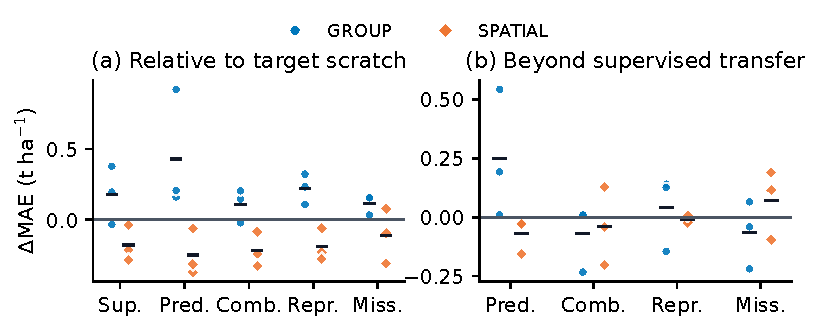
\includegraphics[width=\textwidth]{../figures/final_publication_v4_18/figure_02.pdf}
\caption{Run-level transfer effects in mean absolute error (MAE). Panel (a) compares routes with target scratch; SPATIAL uses one fixed local reference shared across transferred runs. Panel (b) compares routes with run-matched supervised transfer. Negative $\Delta$MAE denotes improvement.}
\label{fig:performance}
\end{figure}

\subsection{Transfer redistributes information use}

Under \group{}, every non-supervised route increases observation-support attribution share. Mean changes range from 0.069 to 0.102, and 72--84\% of sample clusters move upward. Under \spatial{}, combined KD increases the share by 0.048 (95\% bootstrap interval $[0.019,0.075]$), missing-aware training decreases it by 0.021 ($[-0.033,-0.009]$), and the other routes centre near zero. Signed feature changes in the Supplement show compensating shifts among temperature, radiation, and water-balance variables.

\begin{figure}[!t]
\centering
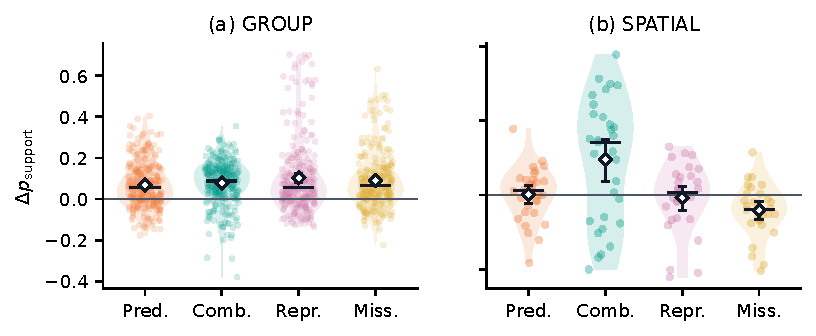
\includegraphics[width=\textwidth]{../figures/final_publication_v4_18/figure_03.pdf}
\caption{Matched observation-support redistribution relative to supervised transfer. Panels (a--b) show GROUP and SPATIAL sample clusters; diamonds and intervals are means with 95\% bootstrap intervals, and bars are medians. Pred., Comb., Repr., and Miss. denote the four transferred routes. Descriptive beeswarms appear in the Supplement.}
\label{fig:redistribution}
\end{figure}

Attribution redistribution is not reducible to predictive performance. GROUP combined KD and prediction KD both increase observation-support attribution yet have different errors. SPATIAL prediction KD improves with near-zero aggregate support shift. The direction and route ordering of attribution redistribution differ across contracts.

\subsection{Attribution redistribution and error change are contract dependent}

A family-adjusted association appears for GROUP prediction KD: $\rho=0.220$, 95\% bootstrap interval $[0.087,0.338]$, Holm $p=0.0016$; trimming gives $\rho=0.232$. One run has the opposite direction, and the other seven tests have estimates from $-0.158$ to 0.148. The attribution--error association therefore varies across routes, contracts, and runs.

\begin{figure}[!t]
\centering
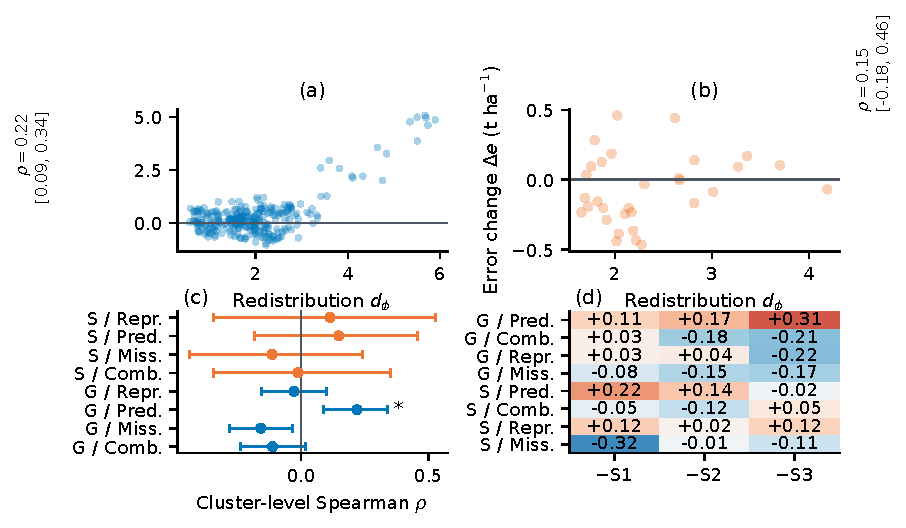
\includegraphics[width=\textwidth]{../figures/final_publication_v4_18/figure_04.pdf}
\caption{Redistribution--error relations. Panels (a--b) show prediction-KD sample clusters; (c) reports eight route--contract tests (*: Holm-adjusted $p<0.05$); (d) omits one run. G/S denote GROUP/SPATIAL; Pred./Comb./Repr./Miss. denote prediction/combined/representation KD and missing-aware training; $-\mathrm{S1}$--$-\mathrm{S3}$ identify the omitted run.}
\label{fig:linkage}
\end{figure}

\subsection{Attribution and finite stress response capture different behaviour}

Across 30 route--contract--run cells, four-group attribution--stress rank agreement averages $-0.040$ (GROUP 0.067; SPATIAL $-0.147$). The top group matches in 30\% of cells. Local contribution allocation and finite function response therefore do not provide the same ranking.

Median replacement moves samples farther from well-represented regions of the training distribution. Mean nearest-neighbour distance rises from 0.759 to 0.922--1.170; stable covariance distance rises from 2.68 to 3.25--5.94. IG meets its completeness criterion for 98.9\% of explanations. Pathwise Taylor meets its local residual criterion in 28 of 180 cases (15.6\%), providing a diagnostic check on the local approximation. These measurements define the operating range of the stress analysis.

\begin{figure}[!t]
\centering
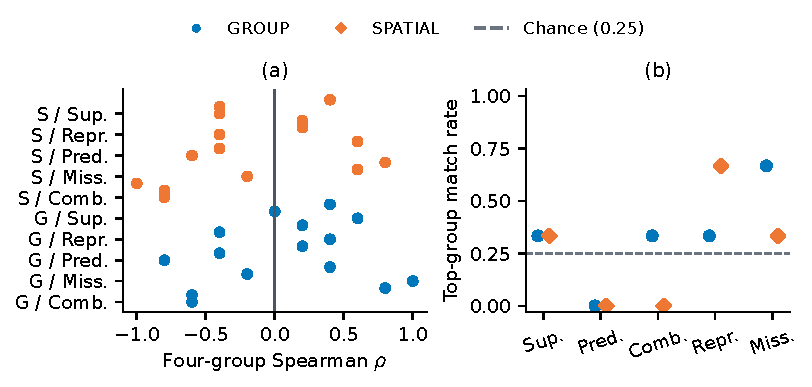
\includegraphics[width=\textwidth]{../figures/final_publication_v4_18/figure_05.pdf}
\caption{Attribution--stress agreement across four disjoint groups: (a) cell-wise Spearman agreement; (b) top-group match by route and contract (dashed line: 0.25 chance). Stress is prediction change per standardised perturbation distance; representative profiles appear in the Supplement.}
\label{fig:stress}
\end{figure}

\FloatBarrier

\section{Discussion}

\begin{table}[t]
\centering
\small
\setlength{\tabcolsep}{3.0pt}
\renewcommand{\arraystretch}{0.94}
\caption{Panels (a)--(e) report Roseworthy, random forest (RF), privileged information, Waite, and behavioural diagnostics. In (a), mean absolute error (MAE) and root mean squared error (RMSE) are in t/ha, coefficient of determination ($R^2$) is dimensionless, and $\Delta$MAE = no-soil route minus no-soil scratch; negative values favour the route. Panel (b) gives joint, branch-average (Avg.), and best-branch MAE. Panel (c) reports run-level MAE and the across-run mean; panel (d) reports run-level MAE under the two Waite protocols. Panel (e) gives attribution--stress ranks, top-group match, Integrated Gradients (IG) completeness, and Taylor local fidelity. Each setting uses its native protocol.}
\label{tab:cross-scale}
\textbf{(a)}\\[-2pt]
\begin{tabular}{@{}lrrrrrrr@{}}
\toprule
Route & \multicolumn{3}{c}{Complete} & \multicolumn{3}{c}{No soil} & $\Delta$MAE\\
 & MAE & RMSE & $R^2$ & MAE & RMSE & $R^2$ & NS--scratch\\
\midrule
Scratch & 0.465 & 0.637 & 0.131 & 0.499 & 0.667 & 0.049 & 0.000\\
Sup. init. & 0.465 & 0.637 & 0.133 & 0.465 & 0.637 & 0.133 & $-0.034$\\
Pred. KD & 0.470 & 0.641 & 0.122 & 0.470 & 0.641 & 0.122 & $-0.029$\\
Repr. KD & 0.473 & 0.644 & 0.112 & 0.473 & 0.644 & 0.112 & $-0.026$\\
Comb. KD & 0.466 & 0.637 & 0.133 & 0.466 & 0.637 & 0.133 & $-0.033$\\
Miss. & 0.468 & 0.639 & 0.125 & 0.468 & 0.639 & 0.125 & $-0.030$\\
\bottomrule
\end{tabular}

\vspace{4pt}
\begin{minipage}[t]{.49\linewidth}
\centering
\scriptsize
\textbf{(b)}\\[-2pt]
\begin{tabular}{@{}lrrr@{}}
\toprule
Condition & Joint & Avg. & Best\\
\midrule
Complete & 0.944 & 1.053 & 1.024\\
15\% missing & 0.920 & 1.015 & 1.004\\
No weather & 1.024 & 1.024 & 1.024\\
\bottomrule
\end{tabular}

\vspace{3pt}
\textbf{(c)}\\[-2pt]
\begin{tabular}{@{}lrrrr@{}}
\toprule
Route & S1 & S2 & S3 & Mean\\
\midrule
Obs. target & 0.935 & 0.580 & 0.863 & 0.793\\
Pseudo & 0.901 & 0.598 & 0.880 & 0.793\\
Blend & 0.886 & 0.583 & 0.871 & 0.780\\
\bottomrule
\end{tabular}

\end{minipage}\hfill
\begin{minipage}[t]{.49\linewidth}
\centering
\scriptsize
\textbf{(d)}\\[-2pt]
\begin{tabular}{@{}lrrr@{}}
\toprule
Protocol & S1 & S2 & S3\\
\midrule
Temporal-forward & 0.691 & 0.698 & 0.685\\
Plot-group & 0.502 & 0.477 & 0.499\\
\bottomrule
\end{tabular}

\vspace{3pt}
\textbf{(e)}\\[-2pt]
\begin{tabular}{@{}lr@{}}
\toprule
Measure & Value\\
\midrule
Rank agreement (mean) & $-0.040$\\
GROUP / SPATIAL & $0.067 / -0.147$\\
Top-group match & 30\%\\
IG completeness & 98.9\%\\
Taylor local fidelity & 28/180 (15.6\%)\\
\bottomrule
\end{tabular}
\end{minipage}
\end{table}

\paragraph{Contract-dependent regional transfer.}
GROUP withholds environments or administrative populations; SPATIAL withholds contiguous locations. They define different target populations and extrapolation demands. Prediction KD helps under SPATIAL and harms under GROUP, with local scratch identifying whether source knowledge adds value. Negative mean SPATIAL $R^2$ separates relative gain from absolute predictive adequacy.

\paragraph{Scale and modality availability at Roseworthy.}
Roseworthy E5 extends modality analysis to a point-level, within-paddock comparison. Complete-input scratch and supervised source-initialised fine-tuning both have MAE 0.465. Without soil, transfer remains at 0.465 while scratch degrades to 0.499. RF means and privileged-information run values further show that route preference varies with learner, missingness pattern, and run. Deployment inputs therefore belong within the transfer contract.

\paragraph{Waite as a protocol comparison.}
At the historical Waite station, temporal-forward and plot-group protocols produce different MAE ranges because they define different prediction tasks. This extends deployment-conditioned evaluation to protocol choice at another agricultural scale.

\paragraph{Multi-view and broader implications.}
Error, attribution, and stress response measure different objects; correlated weather variables and sample-level cancellation may contribute to their weak alignment. Common-sample comparisons show that the three views are complementary.

In a supplementary common-sample comparison with APSIM Next Generation \cite{Holzworth2018APSIMNextGen}, validation-selected weather-only transfer had mean MAE of 0.837 versus 0.948~t/ha under GROUP and 0.990 versus 1.057~t/ha under SPATIAL for the prespecified constrained-input configuration. All paired bootstrap intervals included zero, and sensitivity settings changed the ordering, supporting a complementary prediction role under limited deployment inputs rather than equivalence or general superiority.

These findings motivate local validation and contract-aligned model selection because geography, scale, and input availability can alter the preferred strategy. Preliminary US-to-Brazil observations also indicate effective cross-country transfer under compatible Southern Hemisphere conditions.

\section{Related Work}

\paragraph{Transfer, distillation, and negative transfer.}
Distillation and privileged-information learning transfer richer source supervision \cite{Hinton2015Distillation,LopezPaz2016GeneralizedDistillation,Tian2020CRD}. Agricultural studies show gains with limited target labels, while negative-transfer work frames harm relative to a target learner \cite{Bohra2025KenyaTransfer,Niu2022TransferGapKD,Priyatikanto2023MaizeAdaptation,Wang2019NegativeTransfer}. These studies mainly report aggregate target accuracy within one validation design, leaving route value across target populations unclear. We compare matched GROUP and SPATIAL routes with local scratch and supervised-transfer references.

\paragraph{Structured deployment validation.}
Structured spatial, temporal, and grouped validation shows that partitions change generalisation estimates, applicability, and model selection \cite{Meyer2021AOA,Meyer2022MLMaps,Roberts2017StructuredCV}. This work focuses on predictive scores and applicability, leaving information reliance less directly observed. Our comparisons fix contract, run, sample, feature order, preprocessing, and attribution background.

\begingroup\emergencystretch=1em
\paragraph{Explanation shift and perturbation validity.}
SHAP and IG describe local contributions \cite{Lundberg2017SHAP,Sundararajan2017IntegratedGradients}; explanation-shift and perturbation analyses describe distributional change or finite sensitivity \cite{Kulinski2023ExplainingShift,Mougan2025ExplanationShift}. Conclusions depend on reference data, feature dependence, and intervention design \cite{Aas2021DependentSHAP,Hase2021OODExplainability,Hooker2019ROAR}. We compare attribution movement with matched target-error change on common samples and use OOD checks to bound stress interpretation.
\endgroup

\section{Conclusion}

\paragraph{Limitations.} The primary study covers one cross-crop pair, two contracts, three runs, and a 31-observation SPATIAL test with fixed scratch. Attribution depends on its background, stress on the intervention distribution, and Roseworthy has unresolved public-file correspondence and upstream source identity.

Prediction KD improves SPATIAL transfer but produces negative transfer under GROUP. Error, attribution, and stress are not interchangeable. Realised transfer depends on the model, target, adaptation, and deployment relation, not on a checkpoint alone.

\noindent\textbf{Data and code availability.} Code, configurations, acquisition scripts, and derived tables will be released upon acceptance; restricted raw data will not be redistributed.

\noindent\textbf{Use of generative AI tools.} OpenAI ChatGPT and Codex were used for language polishing and assistance with code drafting. All scientific decisions, analyses, numerical results, references, and final content were reviewed and verified by the authors.

\bibliographystyle{venue/lncs/splncs04}
\bibliography{final_references_v4_18_4_apsim}

\end{document}
